%%% Preamble
\documentclass[	DIV=calc,%
							paper=a4,%
							fontsize=12pt,%
							onecolumn]{scrartcl}	 					% KOMA-article class


\usepackage{lipsum}													% Package to create dummy text
\usepackage[brazil]{babel}										% English language/hyphenation
\usepackage[protrusion=true,expansion=true]{microtype}				% Better typography
\usepackage{amsmath,amsfonts,amsthm}					% Math packages
\usepackage[pdftex]{graphicx}									% Enable pdflatex
\usepackage[svgnames]{xcolor}									% Enabling colors by their 'svgnames'
\usepackage[hang, small,labelfont=bf,up,textfont=it,up]{caption}	% Custom captions under/above floats
\usepackage{epstopdf}												% Converts .eps to .pdf
\usepackage{subfig}													% Subfigures
\usepackage{booktabs}												% Nicer tables
\usepackage{fix-cm}													% Custom fontsizes
\usepackage[utf8]{inputenc}
\usepackage{xcolor}
\usepackage{natbib}
\usepackage[top=2.5cm, bottom=2.5cm, left=2.5cm, right=2.5cm]{geometry}
\usepackage[ddmmyyyy]{datetime}
\addto\captionsenglish{%
	\renewcommand\tablename{Tabela}
	\renewcommand\figurename{Figura}
} 
 

 
%%% Custom sectioning (sectsty package)
\usepackage{sectsty}													% Custom sectioning (see below)
\allsectionsfont{%															% Change font of al section commands
	\usefont{OT1}{phv}{b}{n}%										% bch-b-n: CharterBT-Bold font
	}
\sectionfont{%																% Change font of \section command
	\usefont{OT1}{phv}{b}{n}%										% bch-b-n: CharterBT-Bold font
	}


%%% Headers and footers
\usepackage{fancyhdr}												% Needed to define custom headers/footers
	\pagestyle{fancy}														% Enabling the custom headers/footers
\usepackage{lastpage}	

% Header (empty)
\lhead{}
\chead{}
\rhead{}
% Footer (you may change this to your own needs)

%% ====================================
%% ====================================
%% mude o rodape  do projeto
%% ====================================
%% ====================================

\lfoot{\footnotesize \texttt{Gerenciamento de Configuração de Software} \textbullet ~2ST}


\cfoot{}
\rfoot{\footnotesize página \thepage\ de \pageref{LastPage}}	% "Page 1 of 2"
\renewcommand{\headrulewidth}{0.0pt}
\renewcommand{\footrulewidth}{0.4pt}



%%% Creating an initial of the very first character of the content
\usepackage{lettrine}
\newcommand{\initial}[1]{%
     \lettrine[lines=3,lhang=0.3,nindent=0em]{
     				\color{DarkGoldenrod}
     				{\textsf{#1}}}{}}



%%% Title, author and date metadata
\usepackage{titling}															% For custom titles

\newcommand{\HorRule}{\color{DarkGoldenrod}%			% Creating a horizontal rule
									  	\rule{\linewidth}{1pt}%
										}

\pretitle{\vspace{-30pt} \begin{flushleft} \HorRule 
				\fontsize{50}{50} \usefont{OT1}{phv}{b}{n} \color{DarkRed} \selectfont 
				}

%% ====================================
%% ====================================
%% mude o titulo  do projeto
%% ====================================
%% ====================================

\title{Gerenciamento de Configuração de Software 2ST }					% Title of your article goes here

%% ====================================



\posttitle{\par\end{flushleft}\vskip 0.5em}

\preauthor{\begin{flushleft}
					\large \lineskip 0.5em \usefont{OT1}{phv}{b}{sl} \color{DarkRed}}
\author{Jonata William de Arruda}  	% Author name goes here


\postauthor{\footnotesize \usefont{OT1}{phv}{m}{sl} \color{Black} 
					\\Universidade Tecnológica Federal do Paraná - Câmpus Cornélio Procópio 								% Institution of author
					\par\end{flushleft}\HorRule}

\date{}																				% No date




%%% Begin document
\begin{document}
\maketitle
\thispagestyle{fancy} 	
\thispagestyle{empty}		% Enabling the custom headers/footers for the first page 
% The first character should be within \initial{}




%% ====================================
%% ====================================
%% mude o resumo  do projeto
%% ====================================
%% ====================================
\initial{P}\textbf{lano de Gerenciamento de Configuração de Softwareda 2ST visa especificar o processo para controle de versões, atualizações, distribuições e correções (bugs) relacionado aos produtos de software Klassic da empresa 2ST. Incluso a este documento um guia passo a passo (guideline) de integração a novos desenvolvedores, assim ambientando de forma prática e eficaz as rotinas e processos do desenvolvimento do produto.}

%% ====================================
\begin{figure}
	\centering
	
\includegraphics{utfpr}
\end{figure}

\vspace{3cm}
\centerline{\textit{\textbf{\today}}}

\clearpage
    \renewcommand*\listfigurename{Lista de figuras}
\listoffigures

\renewcommand*\listtablename{Lista de tabelas}
\listoftables




\clearpage
\renewcommand{\contentsname}{Sumário}
\tableofcontents
\clearpage

%% ====================================
%% ====================================
%% Inicio do texto
%% ====================================
%% ====================================
\section{Introdução}
\paragraph{}
O Gerenciamento de Configuração de Software é parte da Engenharia de Software e contém um conjunto de atividades de apoio ao desenvolvimento onde permite que as mudanças inerentes sejam absorvidas pelo projeto de maneira controlada, mantendo a estabilidade na evolução do software, pois mudanças durante o desenvolvimento são inevitáveis.
\paragraph{}
Sendo assim, o objetivo deste documento  é especificar o processo de Gerência de Configuração de Software da empresa 2ST, referente o produto Klassic, afim de atender o mercado que busca por maior qualidade e produtividade no processo de desenvolvimento. Foram criados processos para controlar novas versões, atualizações, correções e distribuições, além de um guia para integração de novos desenvolvedores.

\section{Estado atual}
\paragraph{}
A empresa 2ST atua no ramo de software. Seu perfil de investidores  é alinhado com o mercado e atende as expectativas. Possui carteira de clientes generosa. A equipe de desenvolvimento é composta por 10 integrantes. Possui o produto de software Klassic o qual foi foi desenvolvido por um arquiteto de software que não está mais na organização.
\paragraph{}
Atualmente existem clientes que necessitam de customizações. A customização de um cliente pode não atender outro e há clientes que não necessitam de customizações. O software poderá ser otimizado ou novas funcionalidades poderão ser inseridas: A otimização/nova funcionalidade poderá ser incorporada em todos os clientes. Novas versões poderão ser lançadas.


\section{Requisitos}
\begin{itemize}
	\item Desenvolvido em Java.
	\item Utiliza JPA.
	\item Utiliza PostgreSQL.
	\item Ferramenta IDE NetBeans 8.
	\item Utilza de maneira restrita a geração de código.
	\item Diagramas desenvolvido com Astah.
\end{itemize}

\newpage
\section{Ferramentas}
\paragraph{}
As ferramentas utilizadas para o Gerenciamento de Controle de Software adotados pela empresa 2ST são:

\begin{table}[h!]
\centering
\caption{Ferramentas utilizadas para Controle de Gerenciamento de Software na 2ST}
\label{tabela-ferramentas}
\begin{tabular}{|l|l|}
\hline
Tipo de Ferramenta    & Nome \\ \hline
Controle de Versão     & GitHub     \\ \hline
Controle de Mudança       & Waffle.io     \\ \hline

\end{tabular}
\end{table}

\section{Controle de Versão}
\paragraph{}
Para controlar as versão dos produtos de software é utilizado o GitHub. Através da ferramenta é possível gerenciar todas as mudanças do produto, conferir o autor de cada alteração, criar tags para identificação de versão e rastreablidade, padronizar mensagens de commit, realizar buscas por datas, tags, usuários, versões, entre outros que possam ajudar em uma auditoria, levantamento de métricas e demais necessidades relacionadas ao desenvolvimento do software.

\subsection{Repositório}
\paragraph{}
Para cada produto de software será mantido uma branch "master" onde todo o desenvolvimento do mesmo é contido.
\paragraph{}
Em caso de custimização especifica por um cliente, esta não sendo aproveitada na versão do produto principal, "master", é gerada uma nova branch com o nome do cliente.

\subsection{Baseline}
\paragraph{}
Como mencionado anteriormente a branch principal de cada produto de software terá como rótulo "master", está é a baseline padrão onde manterá o controle de versões seguindo as nomenclaturas adotadas.
\paragraph{}
Em caso de branch gerada ao cliente, esta apresentará a nomenclatura padrão acrescida de uma quarta casa decimal para controle de customização, assim, esta branch continua sendo monitorada pela versão "master" podendo receber suas atualizações, e é possível controlar as versão de customização do cliente especifico.

\subsection{Nomenclatura de versões}
\paragraph{}
Será utilizado da seguinte forma:

\begin{description}
	\item [Version]: Utilizado para informar qual versão encontra se o produto.
	\item [Function]: Alterado apenas quando novas funcionalidades são incorporadas no produto.
	\item [Bugs]: Alterado quando uma correção faz necessário.
	\item [Customize]: Alterado sempre que uma customização especifica de uma cliente é feita. Utilizada apenas em branch de clientes e não na "master".
\end{description}

Exemplo:
\textit{master 1.1.1 }
ou
\textit{cliente A 1.4.10.3}

\subsection{Diagrama}
\paragraph{}
Abaixo é apresentado um exemplo em forma de diagrama do controle de versão utilizando a nomenclatura adotada.
\paragraph{}
Pode se notar a branch "master" sofrendo alterações tanto de novas funcionalidade (Function) quanto de correções (Bugs), ao mesmo tempo uma customização foi necessária sendo criado uma nova branch para o cliente "A". Esta foi clonada da branch "master" com a versão atual. Após a customização, esta branch foi acrescida de em sua nomeclatura (Customize) onde passou a ser rastreada através deste número. 
\paragraph{}
Por fim, a branch "master" incorporou mais algumas funcionalidades desenvolvida e fechou seu ciclo, apresentando uma nova versão da branch, o que logo foi atualizado na branch do cliente A.

\begin{figure}[!h]
	\caption{Diagrama exemplo de Controle de Versão}
	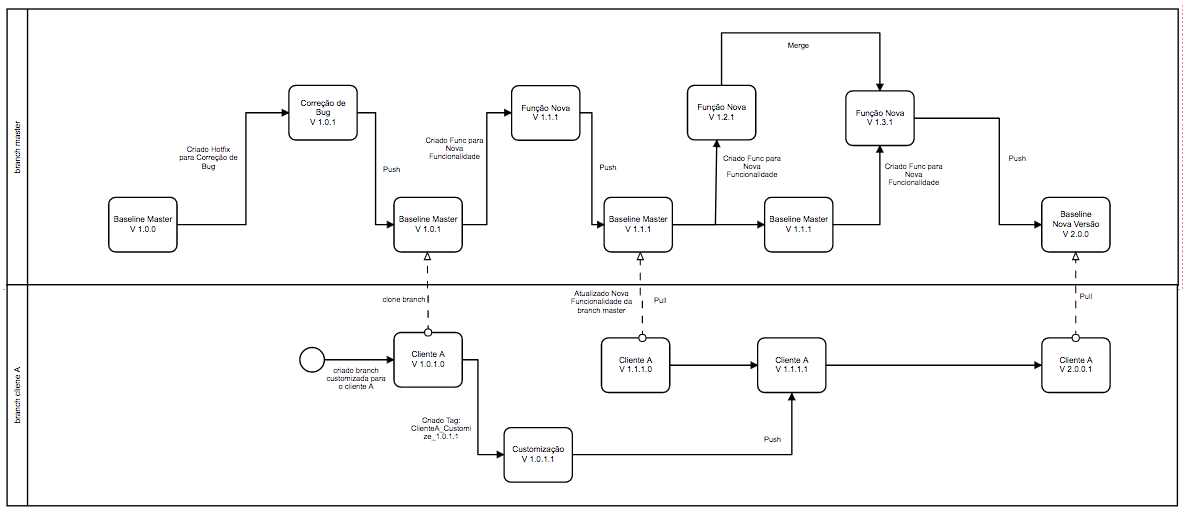
\includegraphics[scale=0.4]{diagrama_branch}
\end{figure}

\subsection{Padrão de Commit}
\paragraph{}
Os "commit" devem seguir um padrão afim de tornar mais fácil a compreensão e integração por parte de novos colaboradores, deixando claro e resumido a alteração aplicada.
\begin{description}
	\item[Nova Distribuição]: Deve ser iniciado com a palavra "Nova Distribuição" seguindo de um espaço e depois "-", mais um espaço e o resumo objetivo da ação executada, neste caso o nome da nova distribuição e o cliente. Exemplo: "Nova Distribuição - sistema de carro cliente Volvo"
	\item[Correções | Bugs]: Deve ser iniciado com a palavra "Correção" seguindo de um espaço e depois "-", mais um espaço e o resumo objetivo da ação executada, neste caso o que foi corrigido. Exemplo: "Correção - Mascara do campo CEP "
	\item[Nova Funcionalidade]: Deve ser iniciado com a palavra "Nova Funcionalidade" seguindo de um espaço e depois "-", mais um espaço e o resumo objetivo da ação executada, neste caso o que seria a nova funcionalidade. Exemplo: "Nova Funcionalidade - Valida CPF"
	\item[Nova Versão]: Deve ser iniciado com a palavra "Nova Versão" seguindo de um espaço e depois "-", mais um espaço e o número da nova versão respeitando a nomenclatura. Exemplo: "Nova Versão - 2.0.0"
\end{description}

\section{Controle de Mudanças}
\paragraph{}
A ferramenta Waffle.io proporciona uma integração com o GitHub o que tornar mais atrativo e eficiente na questão de rastreabilidade e o progresso do desenvolvimento. 
\paragraph{}
Utilizando as Issues gerada para controlar todos os estados de produção da mesma, ou seja, toda movimentação do "card"até sua conclusão, desta forma, foi adotada a ferramenta Waffle.io para controlar as mudanças do produto de software da empresa.

\begin{figure}[!h]
	\caption{Waffle.io - Exemplo de Controle de Mudança utilizando a ferramenta}
	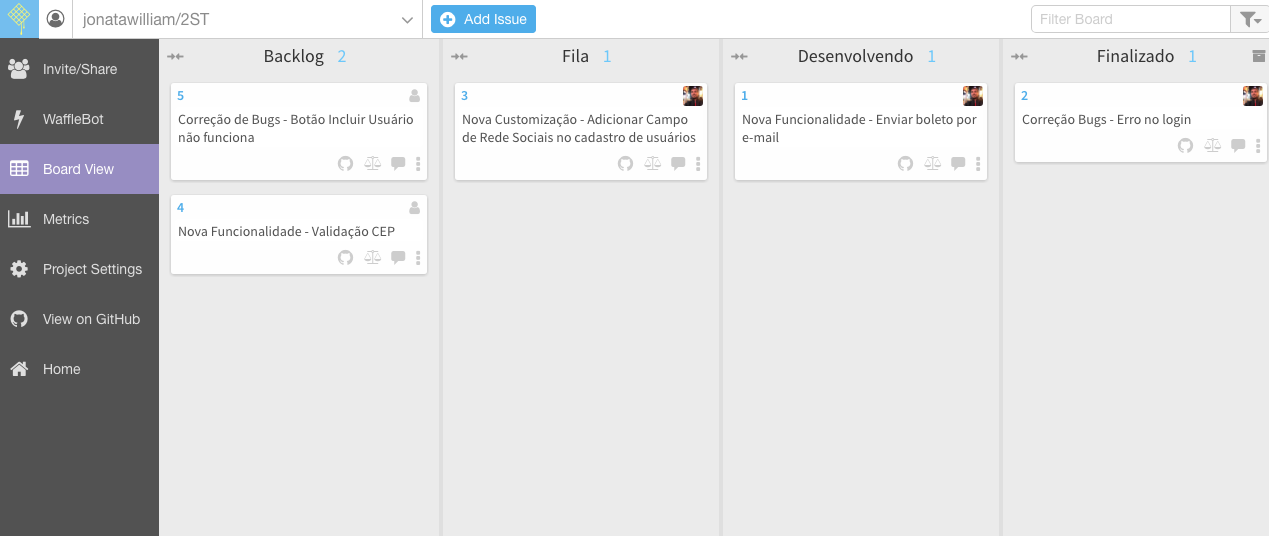
\includegraphics[scale=0.36]{waffleio}
\end{figure}

\newpage
\section{Processos}

\subsection{Papéis}
\paragraph{}
A seguir é descrito a competência que cada membro da equipe deve seguir baseado em seu cargo, estes seguindo uma padrão mencionado na referência \cite{pressman1995engenharia}.
\paragraph{}
Os papéis e suas atribuições são:

\begin{description}
	\item[Analista]: Representa os interesses do cliente e dos usuários finais recolhendo informações dos stakeholders para entender o problema a ser resolvido, capturando os requisitos e definindo suas prioridades.
	\item[Desenvolvedor]: Responsável por desenvolver uma parte do sistema, incluindo a construçãoo de seu design de forma que ele atenda a arquitetura e possivelmente a prototipagem da interface de usuário, e então implementar, executar o teste de unidade, e integrar os componentes que são parte da solução.
	\item[Gerente de Projeto]: Conduz o planejamento do projeto, coordena as interações com os stakeholders e mantêm a equipe de projeto focada em alcançar os objetivos do projeto.
	\item[Cliente]: Grupos de interesse cujas necessidades devem ser atendidas pelo projeto. E um papel que deve ser executado por qualquer pessoa que é, ou será, afetada materialmente pelo resultado do projeto.
\end{description}

\subsection{Novas Distribuição}
\paragraph{}
Uma nova distriuição só é gerada em duas situações:
\begin{enumerate}
	\item Caso seja um novo projeto.
	\item Necessidade de uma customização de alguma versão para um cliente especifico, e somente se esta customização não se aplicar de forma genérica a atender todos os clientes da versão principal (master) do produto. Sendo assim, é gerado uma nova "branch" do produto a partir da versão atual, e ela é acrescida de uma nova casa decimal, onde será controlado o número de customizações que sofreu. 
	\paragraph{}
	Para chegar a tal ponto, deve ser analisado toda a coleta de dados do cliente feita pelo Analista, onde será repassada ao Gerente de Projeto que por sua vez conduzirá e delegará as atividades aos desenvolvedores afim de atender esta nova distribuição.
	\paragraph{}
	Novas distribuições de produtos existentes são evitadas ao máximo afim de manter uma única versão do produto o que facilita sua continuidade e não desperdiçando tempo e desenvolvimento em várias branch, porém sempre que não houver como evitar, uma nova distribuição será criada para atender o cliente.
\end{enumerate}

\subsection{Correções de bugs}
\paragraph{}
O Analista deve analisar o problema relatado pelo cliente / usuário, e verificar se é coerente e verdadeiro, pois alguns relatos de bugs pode ser apenas a má utilização ou falta de conhecimento do mesmo. Caso o Analista identifique que realmente é um problema no produto, o mesmo reporta ao Gerente de Projetos que irá inserir na fila de correções (backlog) com suas devidas prioridades. 
\paragraph{}
Após este passo e seguindo o padrão de nomenclatura, toda correção deve seguir os seguintes passos:
\begin{enumerate}
	\item O Desenvolvedor seleciona o bugs a ser corrigido e aciona o processo de correção.
	\item Abre uma novas hotfix de correção, onde será mantido o número de versão seguindo do número de função e incrementado o número de correções, assim seguindo a nomenclatura. Para este processo, o mesmo deve autenticar a abertura da hotfix com seus dados de login do GitHub que está vinculado a conta da empresa e habilitado a realizar modificações, assim será possível rastrear o que o desenvolvidor realizou neste hotfix.
	\item Assim que corrigido e testado, o mesmo realiza um "commit" seguindo as regras de mensagem para "commit" estabelicidadas neste documento.
	\item Após o "commit" realizado, realiza o "push" para incorporar a branch principal (master) esta correção, e a mesma estar disponível para atualizações nos clientes que utilizam o produto e demais distribuições, principalmente no cliente que relatou o ocorrido.
\end{enumerate}

\subsection{Nova Funcionalidade}
\paragraph{}
Todas a necessidades que o cliente ou o usuário do produto relata, ou seja, coisas que poderiam ter no produto, que poderiam ser de outro jeito e etc, esta direta ou indiretamente, é tratada, analisada e filtrada afim de que o Analista leve ao Gerente de Projeto e equipe de Desenvolvimento e possam discutir sobre o grau de importância e complexidade do mesmo. 
\paragraph{}
Este processo sempre feito para que possam discutir ver se tal funcionalidade não existe, se existe e poderia melhorar ou realmente é algo novo, porém leva sempre em consideração a idéia de construir algo que atenda a todos os clientes dentro da versão principal (master) evitando novas distribuições.
\paragraph{}
Com esta analise feita, segue o processo de desenvolvimento parecido com o de correção:
\begin{enumerate}
	\item O Desenvolvedor seleciona a issue de novo funcionalidade a ser desenvolvida.
	\item Abre uma novas func para novas funcionalidade, onde será mantido o número de versão seguindo e incrementado o  número de função e e mantido o número de correções, assim seguindo a nomenclatura. Para este processo, o mesmo deve autenticar para realizar a abertura da func com seus dados de login do GitHub que está vinculado a conta da empresa e habilitado a realizar modificações, assim será possível rastrear o que o desenvolvidor realizou neste func.
	\item Assim que desenvolvido a nova funcionalidade e testado, o mesmo realiza um "commit" seguindo as regras de mensagem para "commit" estabelicidadas neste documento.
	\item Após o "commit" realizado, realiza o "push" para incorporar a branch principal (master) esta nova funcionalidade, e a mesma estar disponível para atualizações nos clientes que utilizam o produto, e demais distruições.
\end{enumerate}

\subsection{Nova Versão}
\paragraph{}
Sempre que novas funcionalidades são acumuladas e estas acabam não sendo atualizadas, e/ou é definida um ciclo de atualizações e este chega ao fim, uma versão é fechada e da inicio a uma nova versão do produto. Isto tambem para fins marketing. 
\paragraph{}
Para criar uma nova versão, é seguido os passos a seguir:
\begin{enumerate}
	\item Cria se uma nova tag com a versão nova, respeitando a nomenclatura adotada neste documento. Exemplo: Versão anterior 2.3.4. Nova Versão - 3.0.0
	\item Realiza um commit com todas as func e hotfix finalizadas dentro do ciclo especifico para esta nova versão. Utilize o padrão de commit estabeliciddo neste documento.
	\item Realize a atualização desta nova versão tornando disponível para atualização dos clientes.
	\item Em caso de distribuições diferentes, faz necessários a atualização (merge quando necessários) dos mesmo.
\end{enumerate}

\section{Auditoria}
\paragraph{}
Este processo é feito utilizando as ferramentas de Controle de Versão e Controle de Mudança, uma vez que ambas oferece recursos de rastreabilidade. 
\paragraph{}
No Waffle.io e possível rastrear todas a Issues criadas, sabendo desde a hora e data, quem criou, quando foi desenvolvida ou alteraro o card de status, qual data de conclusão, o tempo gasto e mais alguns outros itens.
\paragraph{}
Com a o GitHub, é possível rastrear desde a abertura de uma func, hotfix, criação de branch, tag. Através das tags é possível saber quando foram criado novas versões. Por fazer necessário o login de cada usuário do GitHub, principalmente para participar do diretório dos projetos da empresa, é possível rastrear todas a interações dos usuário, saber pelo log de cada modificação qual usuário que fez, quando e hora, o que foi feito entre outros dados. É possível tambem rastrear modificação seguindo os commit, uma vez que utilizando os padrões adotados por este documento, cada nova função, correção de bugs, nova distribuição e versão do produto torna mais fácil de achar  e filtar dentre os vários commits realizados.

\section{Guideline}
\paragraph{}
Este passo a passo referece a integração do novo colaborador afim do mesmo conseguir instalar o ambiente de desenvolvimento que a empresa adota e posteriormente conseguir colocar em prática este documento de Gerenciamento de Configuração de Software, que trás todos requisitos e passos necessários para compreensão e fluidez do processo de desenvolvimento.

\subsection{Ambiente de desenvolvimento}
\subsubsection{Dependências}
\paragraph{}
Ubuntu 16.04 LTS

\subsubsection{Instalação do Git}
\paragraph{}
Atualize seu OS:
\paragraph{}
\textbf{\colorbox{Silver}{sudo apt update}}
\paragraph{}
Comando para instalar o Git
\paragraph{}
\textbf{\colorbox{Silver}{sudo apt-get install git}}

\subsubsection{Clonar repositório do software Klassic}
\paragraph{}
Git Clone:
\paragraph{}
\textbf{\colorbox{Silver}{git clone https://github.com/jonatawilliam/2ST.git}}
\paragraph{}
Acesse o diretório clonado:
\paragraph{}
\textbf{\colorbox{Silver}{cd 2ST}}
\paragraph{}
Acesse a branch de desenvolvimento desejada, ex:
\paragraph{}
\textbf{\colorbox{Silver}{git checkout 1.0.0}}

\subsubsection{Instalando Java}
\paragraph{}
Insira os repositórios do Java.
\paragraph{}
\textbf{\colorbox{Silver}{sudo apt-get install python-software-properties}}
\textbf{\colorbox{Silver}{sudo add-apt-repository ppa:webupd8team/java}}
\paragraph{}
Atualize o OS.
\paragraph{}
\textbf{\colorbox{Silver}{sudo apt-get update}}
\paragraph{}
Insira os comandos no terminal para instalar a máquina Java
\paragraph{}
\textbf{\colorbox{Silver}{sudo apt-get install oracle-java8-installer}}
\subsubsection{Instalando Maven}
\paragraph{}
Instale o Maven:
\paragraph{}
\textbf{\colorbox{Silver}{sudo apt-get install maven}}
\paragraph{}
Instale as dependências do projeto através do Maven:
\paragraph{}
\textbf{\colorbox{Silver}{mvn dependency:go-offline}}
\textbf{\colorbox{Silver}{mvn install}}
\paragraph{}
\textbf{\colorbox{Silver}{mvn dependency:go-offline}}
\textbf{\colorbox{Silver}{mvn install}}
\subsubsection{Instalando SGBD e configurando Banco de Dados}
\paragraph{}
Instale o SGBD PostgreSql:
\paragraph{}
\textbf{\colorbox{Silver}{sudo apt-get install postgresql postgresql-contrib}}
\paragraph{}
Cria a database:
\paragraph{}
\textbf{\colorbox{Silver}{sudo psql -U postgres -c ’CREATE DATABASE klassic;’}}
\paragraph{}
Inicialize o banco:
\paragraph{}
\textbf{\colorbox{Silver}{sudo psql -U postgres -d aula -a -f Scripts/Database.txt}}
\paragraph{}
Certifique-se que dentro do arquivo src/main/resources/META-INF/persistence.xml as
propriedades jdbc.user e jdbc.password estejam corretas de acordo com o seu banco de
dados.
\subsubsection{Próximo passo}
\paragraph{}
A partir deste ponto, segue se todos os processos descritos anteriormente neste documento para poder iniciar o trabalho de desenvolvimento do produto Klassic.
\paragraph{}
No repositório do GitHub está descritos a Guideline com todos os pontos chaves deste documento no que se refere ao papel do desenvolvedor, assim possibilitando ao novo colaborado ter mais uma fonte de informações sobre como proceder com o seu trabalho e ao colaborado que faz parte da empresa, consultar sempre que necesário.


\newpage
\section{Referências bibliográficas}
\bibliographystyle{ieeetr}
\bibliography{referencias} 






\end{document}

